\section{Introduction}
\subsection{Initial situation}
The openETCS project has the goal to develop a semi-formal followed by a strictly formal OBU model realizing
functionalities of the UNISIG SRS-SUBSET-026, baseline 3, required for running on the ETCS level 2 of the
Utrecht-Amsterdam track. The purpose of this formal model is to increase and spread consistent understanding of the
subset, where it can be used as an artifact for testing, analyzing, verification and validation and also for further
development purposes by industrial actors. This shall be achieved within a framework that is based on an open source
concept. The ETCS On Board Unit EVC software model depicted in Figure 1 will be the focus of the software assessment
according to the EN 50128:2011.

 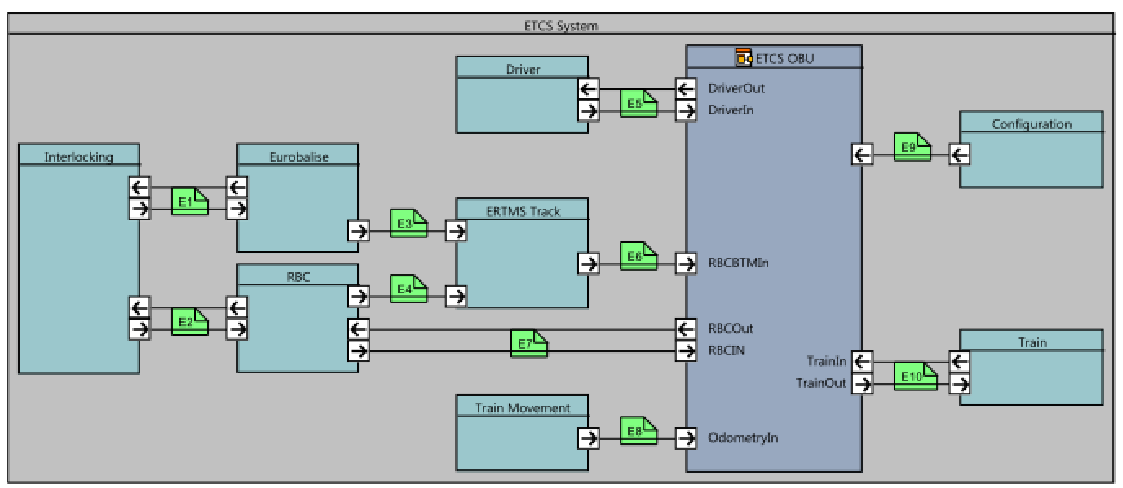
\includegraphics[width=14.552cm,height=6.35cm]{images/toplevelarchitecture.pdf} 

Figure 1: Top level architecture view of the ETCS OBU


\bigskip

\subsection{Scope of the assessment}
The scope of the assessment will cover three main categories of the openETCS software development. These are:

\liststyleLiv
\begin{itemize}
\item Project and Software Quality assurance 
\item Verification \& Validation and 
\item Safety 
\end{itemize}

\bigskip

\subsection{Contents of the assessment and issues of concern}
The purpose of this assessment is to answer the following questions relating to software development:

1. What measures have been taken to satisfy EN 50128?

2. Are the measures taken for satisfying EN 50128 SIL 4 sufficient?

3. Does the agile development methodology applied in this project affect these measures taken for satisfying EN 50128?


\bigskip

\subsection{Assessment conditions and exceptions}
It should be noted:

{}-- The ETCS OBU software model has been developed with the closed source SCADE Suite of the company ESTEREL Technology and the
code generated is SIL4 certified. Hence only the deliverables of the openETCS Tool chain will have the scope of the
assessment.

{}-- HW-Integration is out of the scope of the assessment

\subsection{Documents for the software life cycle
and software creation}
The following documents, which describe the software creation process, have been made available to the expert assessors.


\bigskip


\begin{figure}
\label{documentmapping} 
\centering
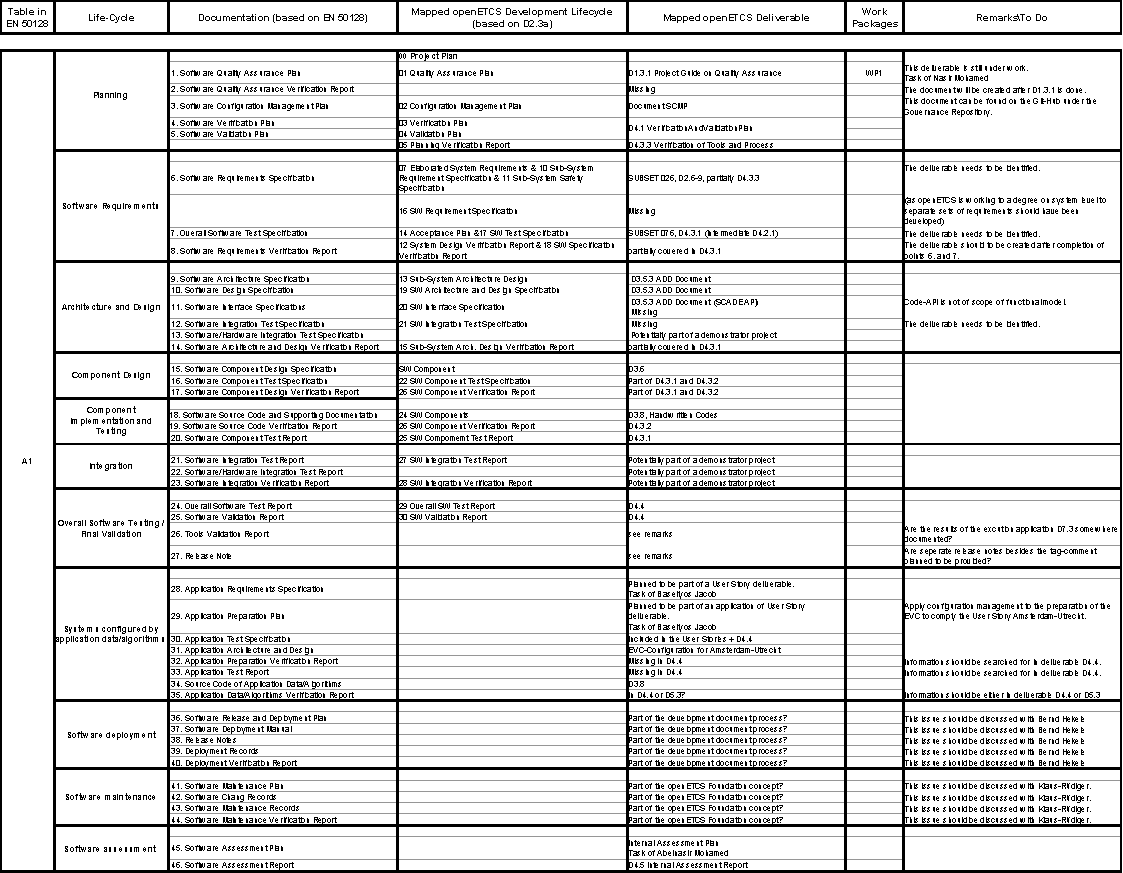
\includegraphics[width=21.001cm,height=16.341cm,angle=-90]{../images/documentmapping.pdf}
\captionof{figure}{Mapping of openETCS Documents to the CENELEC Lifecycle}
\end{figure}


\end{document}
